%& -shell-escape
\documentclass[a4paper,11pt]{article}
\usepackage[latin1]{inputenc}
\usepackage[T1]{fontenc}
\usepackage[italian]{babel}
\usepackage{graphics}

\author{Alfano Emanuele \\ Badalamenti Filippo \\ Vitti Gabriele}


\newcommand{\DHTable}{
	\begin{tabular}{c|c|c|c|c|}
		\cline{2-5} &
		\multicolumn{2}{|c|}{$A_z(\theta,d)$} &
		\multicolumn{2}{|c|}{$A_x(\alpha,a)$} \\
		\hline
		\multicolumn{1}{|c|}{$R_1$} &  &  &  &  \\
		\hline
		\multicolumn{1}{|c|}{R2} &  &  &  &  \\
		\hline
		\multicolumn{1}{|c|}{R3} &  &  &  &  \\
		\hline
	\end{tabular}
}


\begin{document}
\title{Cinematiche Dirette Robot}
\maketitle
\pagebreak

\section*{Cartesiano}
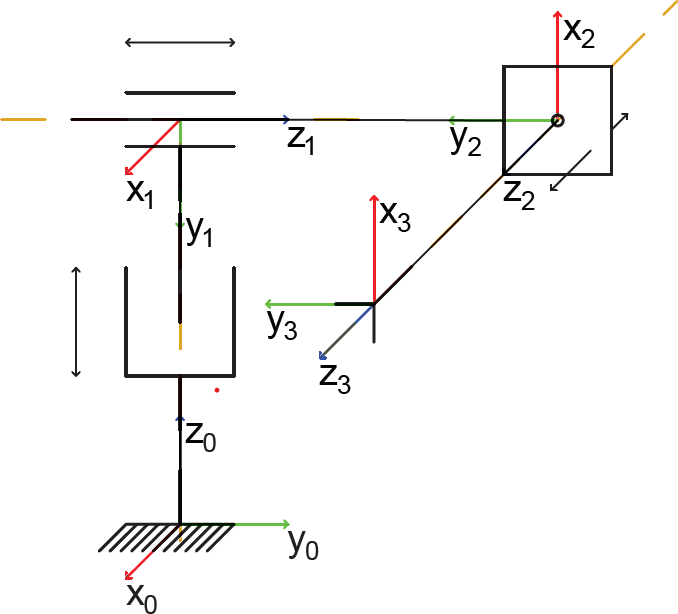
\includegraphics{Sorgenti/Strutture/Cartesiano.png}
\begin{tabular}{c|c|c|c|c|}
            \cline{2-5} &
            \multicolumn{2}{|c|}{$A_z(\theta,d)$} &
            \multicolumn{2}{|c|}{$A_x(\alpha,a)$} \\
            \hline
        \multicolumn{1}{|c|}{$R_1$} & $0$ & $q_{1}$ & $-{{\pi}\over{2}}$ & $0$ \\
            \hline
        \multicolumn{1}{|c|}{$R_2$} & $-{{\pi}\over{2}}$ & $q_{2}$ & $-{{\pi}\over{2}}$ & $0$ \\
            \hline
        \multicolumn{1}{|c|}{$R_3$} & $0$ & $q_{3}$ & $0$ & $0$ \\
            \hline
\end{tabular}


\section*{Cilindrico}
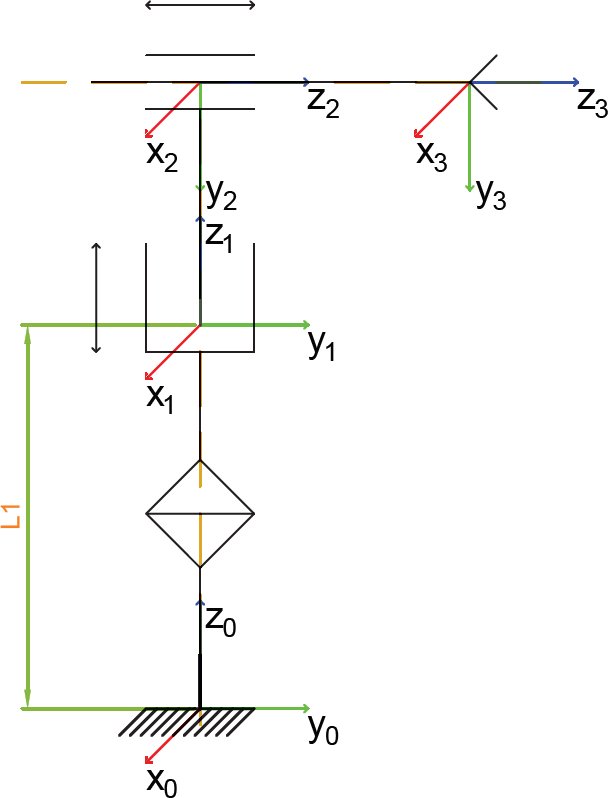
\includegraphics{Sorgenti/Strutture/Cilindrico.png}
\begin{tabular}{c|c|c|c|c|}
            \cline{2-5} &
            \multicolumn{2}{|c|}{$A_z(\theta,d)$} &
            \multicolumn{2}{|c|}{$A_x(\alpha,a)$} \\
            \hline
        \multicolumn{1}{|c|}{$R_1$} & $q_{1}$ & $0$ & $0$ & $D_{1}$ \\
            \hline
        \multicolumn{1}{|c|}{$R_2$} & $q_{2}$ & $0$ & $0$ & $D_{2}$ \\
            \hline
        \multicolumn{1}{|c|}{$R_3$} & $q_{3}$ & $0$ & $0$ & $D_{3}$ \\
            \hline
\end{tabular}


\section*{RRR Planare}
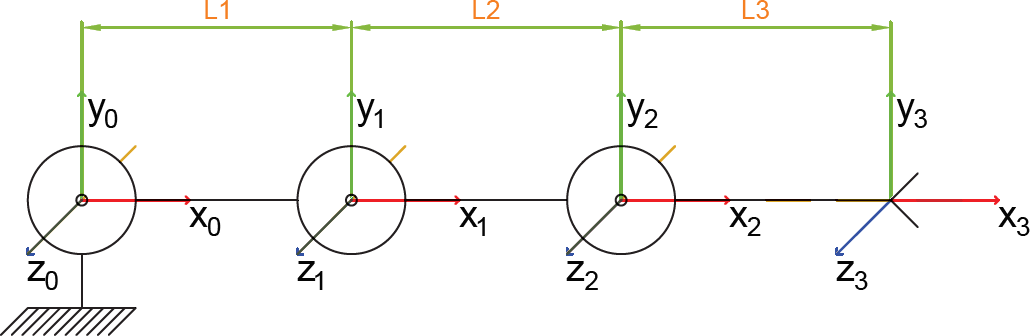
\includegraphics{Sorgenti/Strutture/RRRplanare.png}
\begin{tabular}{c|c|c|c|c|}  
            \cline{2-5} &
            \multicolumn{2}{|c|}{$A_z(\theta,d)$} &
            \multicolumn{2}{|c|}{$A_x(\alpha,a)$} \\
            \hline
        \multicolumn{1}{|c|}{$R_1$} & $q_{1}$ & $0$ & $0$ & $D_{1}$ \\
            \hline
        \multicolumn{1}{|c|}{$R_2$} & $q_{2}$ & $0$ & $0$ & $D_{2}$ \\
            \hline
        \multicolumn{1}{|c|}{$R_3$} & $q_{3}$ & $0$ & $0$ & $D_{3}$ \\
            \hline
\end{tabular}


\section*{Sferico 1}
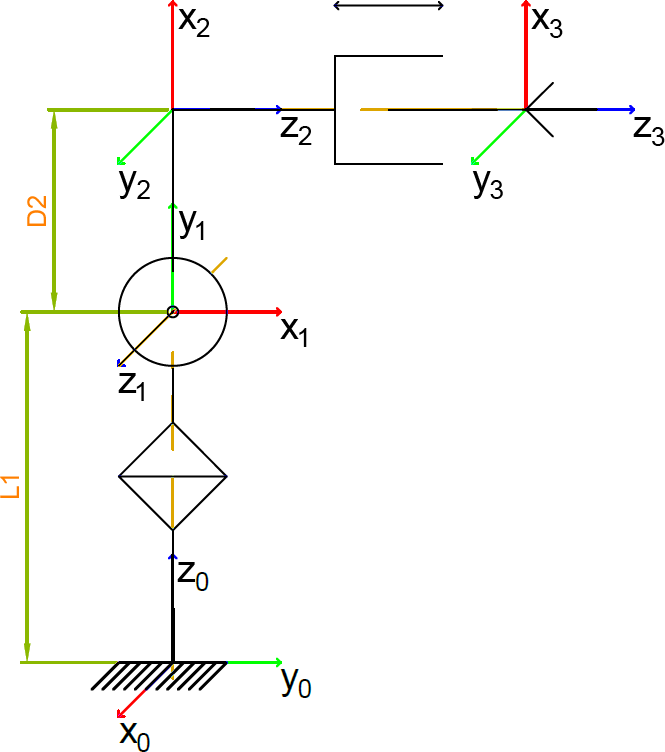
\includegraphics{Sorgenti/Strutture/Sferico1.png}
\begin{tabular}{c|c|c|c|c|}
            \cline{2-5} &
            \multicolumn{2}{|c|}{$A_z(\theta,d)$} &
            \multicolumn{2}{|c|}{$A_x(\alpha,a)$} \\
            \hline
        \multicolumn{1}{|c|}{$R_1$} & $q_{1}$ & $0$ & $0$ & $D_{1}$ \\
            \hline
        \multicolumn{1}{|c|}{$R_2$} & $q_{2}$ & $0$ & $0$ & $D_{2}$ \\
            \hline
        \multicolumn{1}{|c|}{$R_3$} & $q_{3}$ & $0$ & $0$ & $D_{3}$ \\
            \hline
\end{tabular}


\section*{Sferico di Stanford}
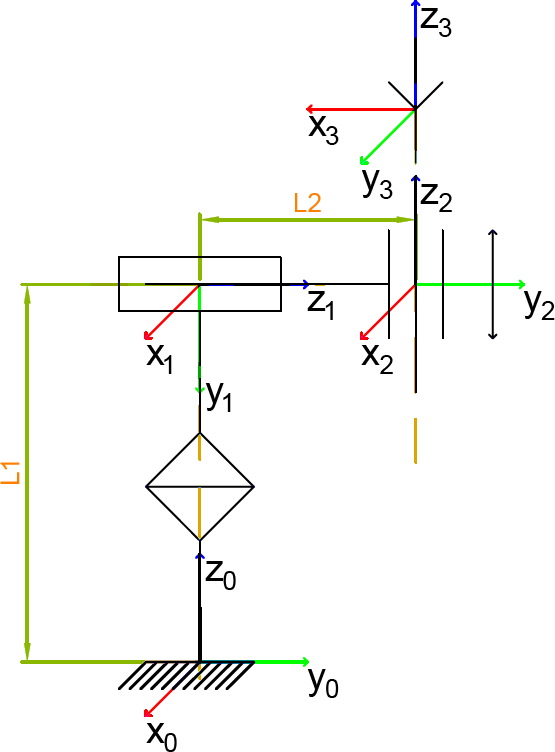
\includegraphics{Sorgenti/Strutture/SfericoStanford.png}
\begin{tabular}{c|c|c|c|c|}
            \cline{2-5} &
            \multicolumn{2}{|c|}{$A_z(\theta,d)$} &
            \multicolumn{2}{|c|}{$A_x(\alpha,a)$} \\
            \hline
        \multicolumn{1}{|c|}{$R_1$} & $q_{1}$ & $0$ & $0$ & $D_{1}$ \\
            \hline
        \multicolumn{1}{|c|}{$R_2$} & $q_{2}$ & $0$ & $0$ & $D_{2}$ \\
            \hline
        \multicolumn{1}{|c|}{$R_3$} & $q_{3}$ & $0$ & $0$ & $D_{3}$ \\
            \hline
\end{tabular}


\section*{Antropomorfo}
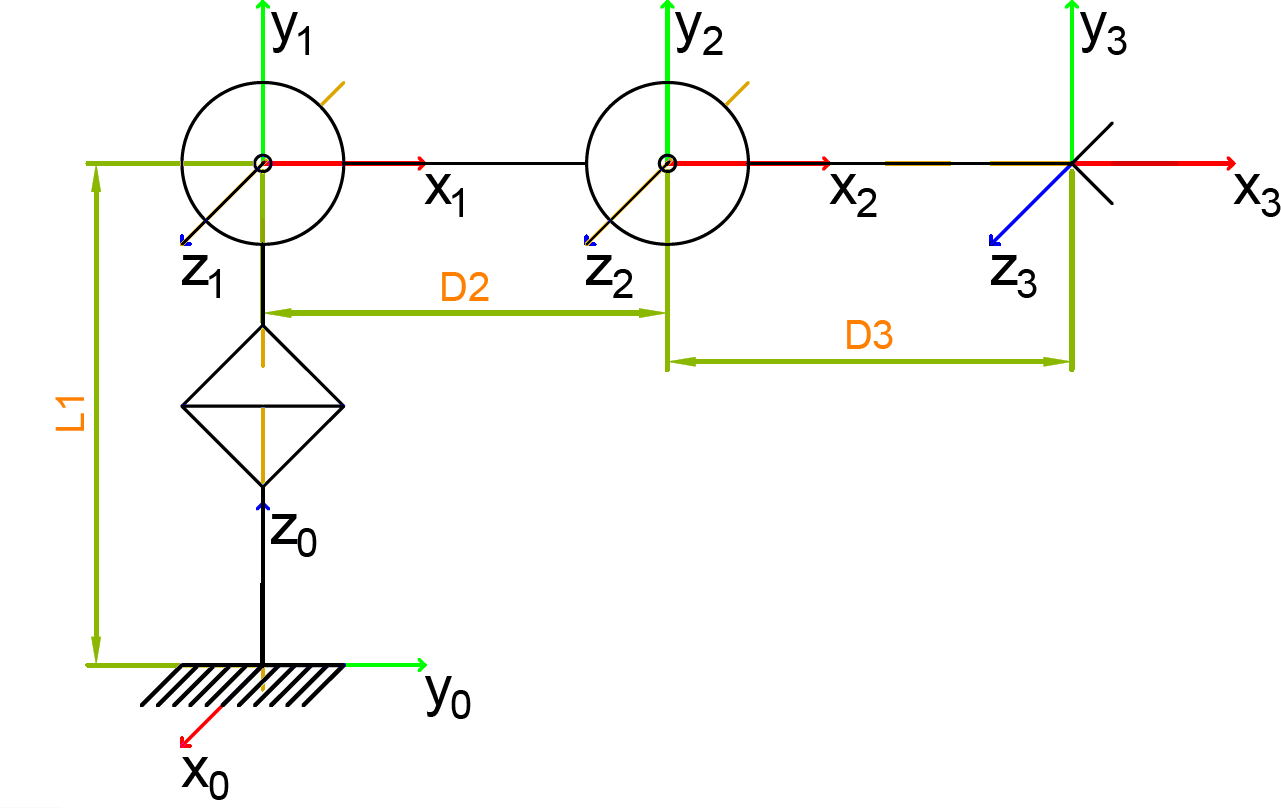
\includegraphics{Sorgenti/Strutture/Antropomorfo.png}
\begin{tabular}{c|c|c|c|c|}
            \cline{2-5} &
            \multicolumn{2}{|c|}{$A_z(\theta,d)$} &
            \multicolumn{2}{|c|}{$A_x(\alpha,a)$} \\
            \hline
        \multicolumn{1}{|c|}{$R_1$} & $q_{1}$ & $0$ & $0$ & $D_{1}$ \\
            \hline
        \multicolumn{1}{|c|}{$R_2$} & $q_{2}$ & $0$ & $0$ & $D_{2}$ \\
            \hline
        \multicolumn{1}{|c|}{$R_3$} & $q_{3}$ & $0$ & $0$ & $D_{3}$ \\
            \hline
\end{tabular}


\section*{Polso Sferico}
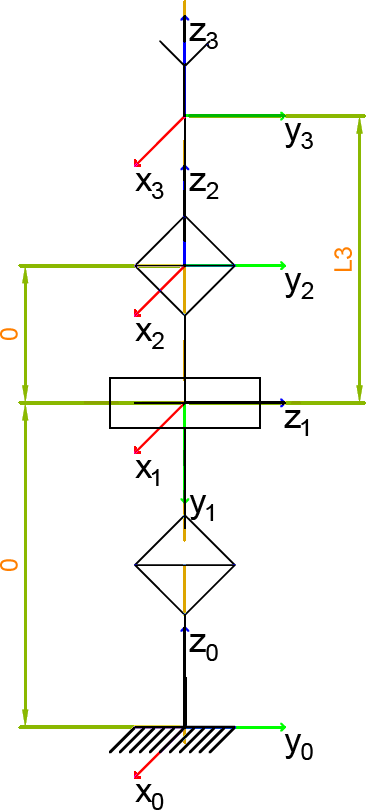
\includegraphics{Sorgenti/Strutture/PolsoSferico.png}
\begin{tabular}{c|c|c|c|c|}
            \cline{2-5} &
            \multicolumn{2}{|c|}{$A_z(\theta,d)$} &
            \multicolumn{2}{|c|}{$A_x(\alpha,a)$} \\
            \hline
        \multicolumn{1}{|c|}{$R_1$} & $q_{1}$ & $0$ & $0$ & $D_{1}$ \\
            \hline
        \multicolumn{1}{|c|}{$R_2$} & $q_{2}$ & $0$ & $0$ & $D_{2}$ \\
            \hline
        \multicolumn{1}{|c|}{$R_3$} & $q_{3}$ & $0$ & $0$ & $D_{3}$ \\
            \hline
\end{tabular}


\section*{Cartesiano con Polso}
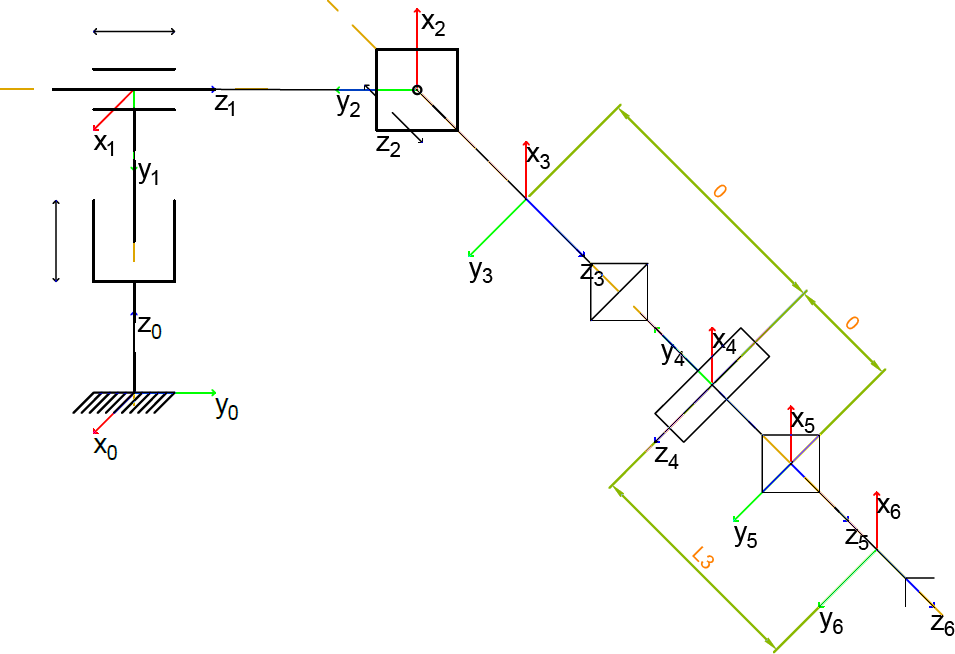
\includegraphics{Sorgenti/Strutture+Polso/Cartesiano+p.png}
\begin{tabular}{c|c|c|c|c|}
            \cline{2-5} &
            \multicolumn{2}{|c|}{$A_z(\theta,d)$} &
            \multicolumn{2}{|c|}{$A_x(\alpha,a)$} \\
            \hline
        \multicolumn{1}{|c|}{$R_1$} & $q_{1}$ & $0$ & $0$ & $D_{1}$ \\
            \hline
        \multicolumn{1}{|c|}{$R_2$} & $q_{2}$ & $0$ & $0$ & $D_{2}$ \\
            \hline
        \multicolumn{1}{|c|}{$R_3$} & $q_{3}$ & $0$ & $0$ & $D_{3}$ \\
            \hline
\end{tabular}


\section*{Cilindrico con Polso}
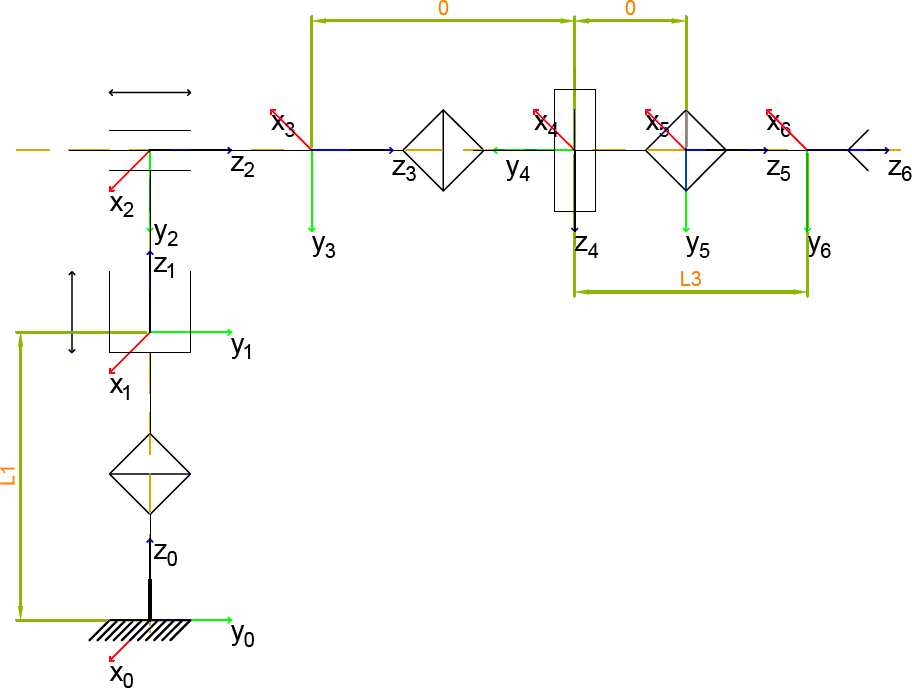
\includegraphics{Sorgenti/Strutture+Polso/Cilindrico+p.png}
\begin{tabular}{c|c|c|c|c|}  
            \cline{2-5} &
            \multicolumn{2}{|c|}{$A_z(\theta,d)$} &
            \multicolumn{2}{|c|}{$A_x(\alpha,a)$} \\
            \hline
        \multicolumn{1}{|c|}{$R_1$} & $q_{1}$ & $L_{1}$ & $0$ & $0$ \\
            \hline
        \multicolumn{1}{|c|}{$R_2$} & $0$ & $q_{2}$ & $-{{\pi}\over{2}}$ & $0$ \\
            \hline
        \multicolumn{1}{|c|}{$R_3$} & $0$ & $q_{3}$ & $0$ & $0$ \\
            \hline
        \multicolumn{1}{|c|}{$R_4$} & $q_{4}$ & $0$ & $-{{\pi}\over{2}}$ & $0$ \\
            \hline
        \multicolumn{1}{|c|}{$R_5$} & $q_{5}$ & $0$ & ${{\pi}\over{2}}$ & $0$ \\
            \hline
        \multicolumn{1}{|c|}{$R_6$} & $q_{6}$ & $L_{6}$ & $0$ & $0$ \\
            \hline
\end{tabular}


\section*{RRR Planare con Polso}
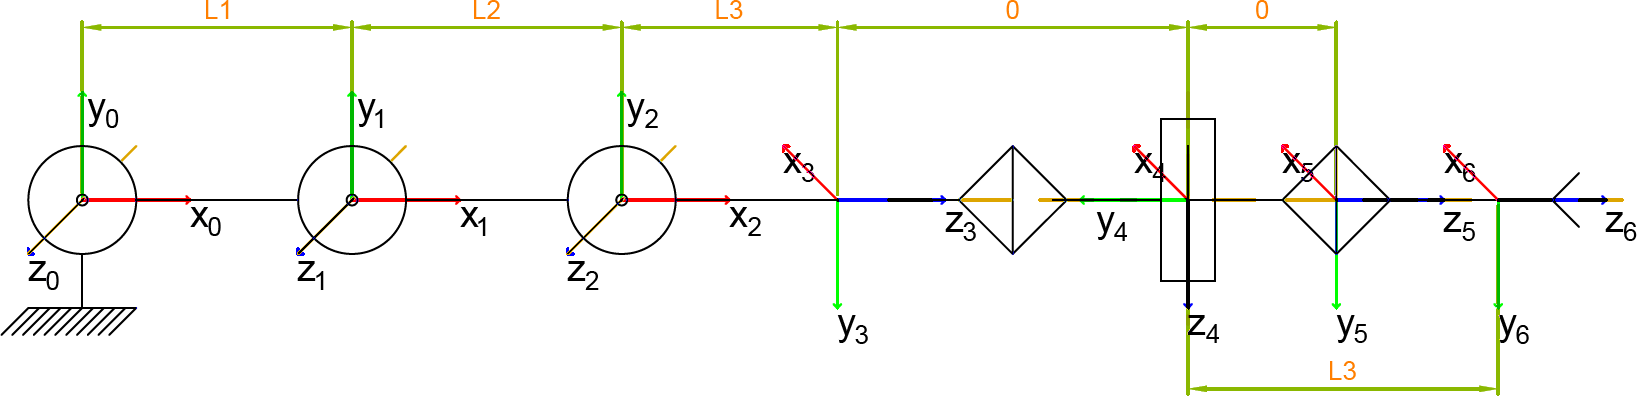
\includegraphics{Sorgenti/Strutture+Polso/RRRplanare+p.png}
\begin{tabular}{c|c|c|c|c|}  
            \cline{2-5} &
            \multicolumn{2}{|c|}{$A_z(\theta,d)$} &
            \multicolumn{2}{|c|}{$A_x(\alpha,a)$} \\
            \hline
        \multicolumn{1}{|c|}{$R_1$} & $q_{1}$ & $0$ & $0$ & $D_{1}$ \\
            \hline
        \multicolumn{1}{|c|}{$R_2$} & $q_{2}$ & $0$ & $0$ & $D_{2}$ \\
            \hline
        \multicolumn{1}{|c|}{$R_3$} & $q_{3}$ & $0$ & $0$ & $D_{3}$ \\
            \hline
\end{tabular}


\section*{Sferico 1 con Polso}
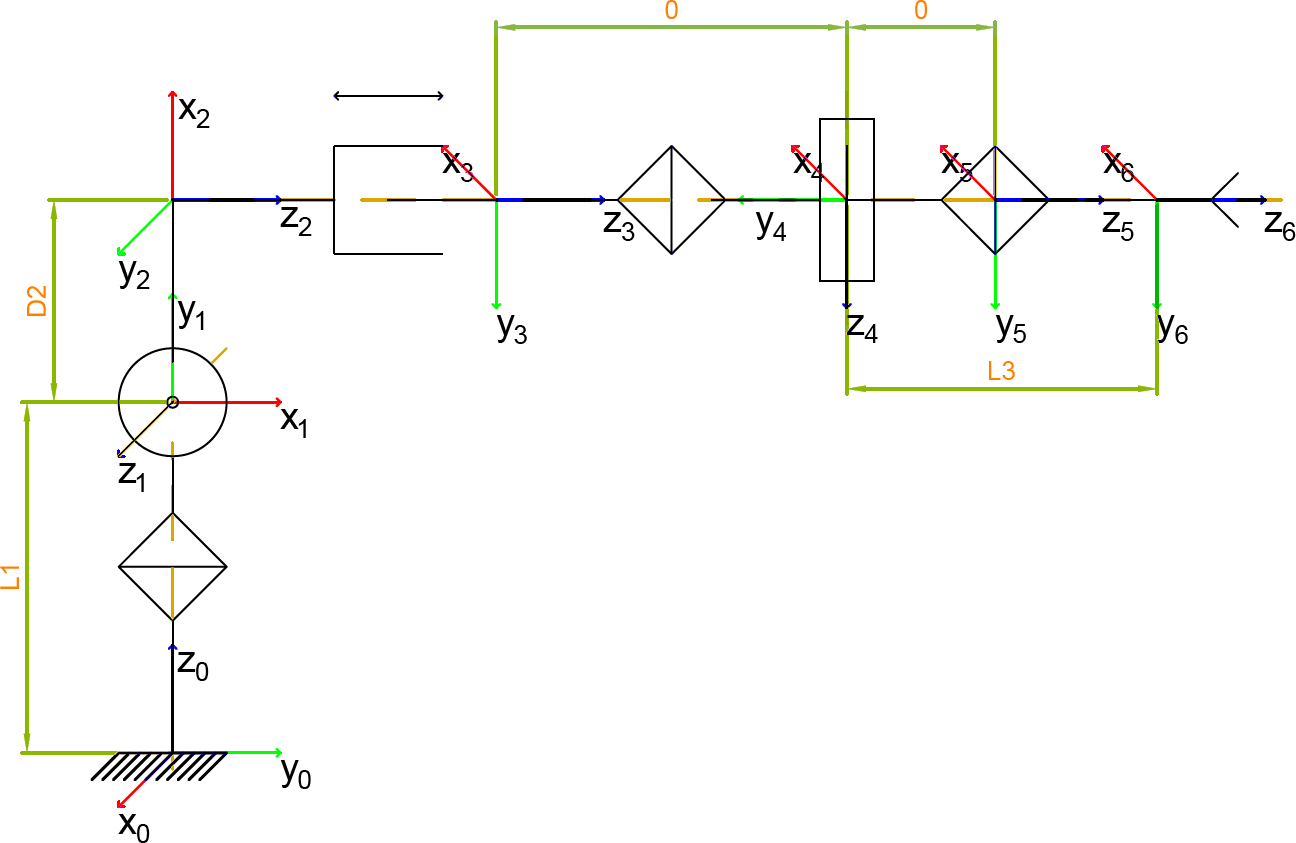
\includegraphics{Sorgenti/Strutture+Polso/Sferico1+p.png}
\begin{tabular}{c|c|c|c|c|}
            \cline{2-5} &
            \multicolumn{2}{|c|}{$A_z(\theta,d)$} &
            \multicolumn{2}{|c|}{$A_x(\alpha,a)$} \\
            \hline
        \multicolumn{1}{|c|}{$R_1$} & $q_{1}$ & $0$ & $0$ & $D_{1}$ \\
            \hline
        \multicolumn{1}{|c|}{$R_2$} & $q_{2}$ & $0$ & $0$ & $D_{2}$ \\
            \hline
        \multicolumn{1}{|c|}{$R_3$} & $q_{3}$ & $0$ & $0$ & $D_{3}$ \\
            \hline
\end{tabular}
$$\pmatrix{-\cos _{q_{1}}\,\cos _{q_{2}}\,\sin _{q_{4}}\,\sin _{q_{6}
 }+\sin _{q_{1}}\,\cos _{q_{4}}\,\sin _{q_{6}}-\cos _{q_{1}}\,\sin _{
 q_{2}}\,\sin _{q_{5}}\,\cos _{q_{6}}+\sin _{q_{1}}\,\sin _{q_{4}}\,
 \cos _{q_{5}}\,\cos _{q_{6}}+\cos _{q_{1}}\,\cos _{q_{2}}\,\cos _{
 q_{4}}\,\cos _{q_{5}}\,\cos _{q_{6}}&\cos _{q_{1}}\,\sin _{q_{2}}\,
 \sin _{q_{5}}\,\sin _{q_{6}}-\sin _{q_{1}}\,\sin _{q_{4}}\,\cos _{
 q_{5}}\,\sin _{q_{6}}-\cos _{q_{1}}\,\cos _{q_{2}}\,\cos _{q_{4}}\,
 \cos _{q_{5}}\,\sin _{q_{6}}-\cos _{q_{1}}\,\cos _{q_{2}}\,\sin _{
 q_{4}}\,\cos _{q_{6}}+\sin _{q_{1}}\,\cos _{q_{4}}\,\cos _{q_{6}}&
 \sin _{q_{1}}\,\sin _{q_{4}}\,\sin _{q_{5}}+\cos _{q_{1}}\,\cos _{
 q_{2}}\,\cos _{q_{4}}\,\sin _{q_{5}}+\cos _{q_{1}}\,\sin _{q_{2}}\,
 \cos _{q_{5}}&L_{6}\,\sin _{q_{1}}\,\sin _{q_{4}}\,\sin _{q_{5}}+
 L_{6}\,\cos _{q_{1}}\,\cos _{q_{2}}\,\cos _{q_{4}}\,\sin _{q_{5}}+
 L_{6}\,\cos _{q_{1}}\,\sin _{q_{2}}\,\cos _{q_{5}}+\cos _{q_{1}}\,
 \sin _{q_{2}}\,q_{3}+D_{2}\,\cos _{q_{1}}\,\cos _{q_{2}}\cr -\sin _{
 q_{1}}\,\cos _{q_{2}}\,\sin _{q_{4}}\,\sin _{q_{6}}-\cos _{q_{1}}\,
 \cos _{q_{4}}\,\sin _{q_{6}}-\sin _{q_{1}}\,\sin _{q_{2}}\,\sin _{
 q_{5}}\,\cos _{q_{6}}-\cos _{q_{1}}\,\sin _{q_{4}}\,\cos _{q_{5}}\,
 \cos _{q_{6}}+\sin _{q_{1}}\,\cos _{q_{2}}\,\cos _{q_{4}}\,\cos _{
 q_{5}}\,\cos _{q_{6}}&\sin _{q_{1}}\,\sin _{q_{2}}\,\sin _{q_{5}}\,
 \sin _{q_{6}}+\cos _{q_{1}}\,\sin _{q_{4}}\,\cos _{q_{5}}\,\sin _{
 q_{6}}-\sin _{q_{1}}\,\cos _{q_{2}}\,\cos _{q_{4}}\,\cos _{q_{5}}\,
 \sin _{q_{6}}-\sin _{q_{1}}\,\cos _{q_{2}}\,\sin _{q_{4}}\,\cos _{
 q_{6}}-\cos _{q_{1}}\,\cos _{q_{4}}\,\cos _{q_{6}}&-\cos _{q_{1}}\,
 \sin _{q_{4}}\,\sin _{q_{5}}+\sin _{q_{1}}\,\cos _{q_{2}}\,\cos _{
 q_{4}}\,\sin _{q_{5}}+\sin _{q_{1}}\,\sin _{q_{2}}\,\cos _{q_{5}}&-
 L_{6}\,\cos _{q_{1}}\,\sin _{q_{4}}\,\sin _{q_{5}}+L_{6}\,\sin _{
 q_{1}}\,\cos _{q_{2}}\,\cos _{q_{4}}\,\sin _{q_{5}}+L_{6}\,\sin _{
 q_{1}}\,\sin _{q_{2}}\,\cos _{q_{5}}+\sin _{q_{1}}\,\sin _{q_{2}}\,
 q_{3}+D_{2}\,\sin _{q_{1}}\,\cos _{q_{2}}\cr -\sin _{q_{2}}\,\sin _{
 q_{4}}\,\sin _{q_{6}}+\cos _{q_{2}}\,\sin _{q_{5}}\,\cos _{q_{6}}+
 \sin _{q_{2}}\,\cos _{q_{4}}\,\cos _{q_{5}}\,\cos _{q_{6}}&-\cos _{
 q_{2}}\,\sin _{q_{5}}\,\sin _{q_{6}}-\sin _{q_{2}}\,\cos _{q_{4}}\,
 \cos _{q_{5}}\,\sin _{q_{6}}-\sin _{q_{2}}\,\sin _{q_{4}}\,\cos _{
 q_{6}}&\sin _{q_{2}}\,\cos _{q_{4}}\,\sin _{q_{5}}-\cos _{q_{2}}\,
 \cos _{q_{5}}&L_{6}\,\sin _{q_{2}}\,\cos _{q_{4}}\,\sin _{q_{5}}-
 L_{6}\,\cos _{q_{2}}\,\cos _{q_{5}}-\cos _{q_{2}}\,q_{3}+D_{2}\,
 \sin _{q_{2}}+L_{1}\cr 0&0&0&1\cr }$$


\section*{Sferico di Stanford con Polso}
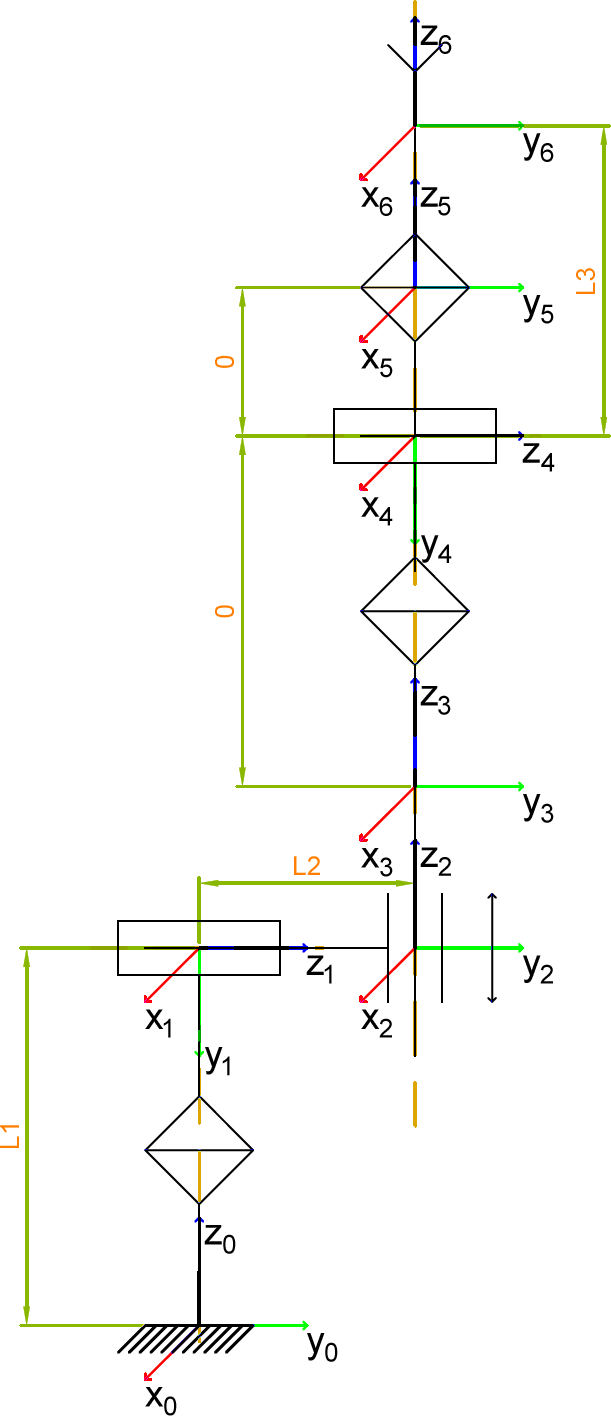
\includegraphics{Sorgenti/Strutture+Polso/SfericoStanford+p.png}
\begin{tabular}{c|c|c|c|c|}
            \cline{2-5} &
            \multicolumn{2}{|c|}{$A_z(\theta,d)$} &
            \multicolumn{2}{|c|}{$A_x(\alpha,a)$} \\
            \hline
        \multicolumn{1}{|c|}{$R_1$} & $q_{1}$ & $0$ & $0$ & $D_{1}$ \\
            \hline
        \multicolumn{1}{|c|}{$R_2$} & $q_{2}$ & $0$ & $0$ & $D_{2}$ \\
            \hline
        \multicolumn{1}{|c|}{$R_3$} & $q_{3}$ & $0$ & $0$ & $D_{3}$ \\
            \hline
\end{tabular}


\section*{Antropomorfo con Polso}
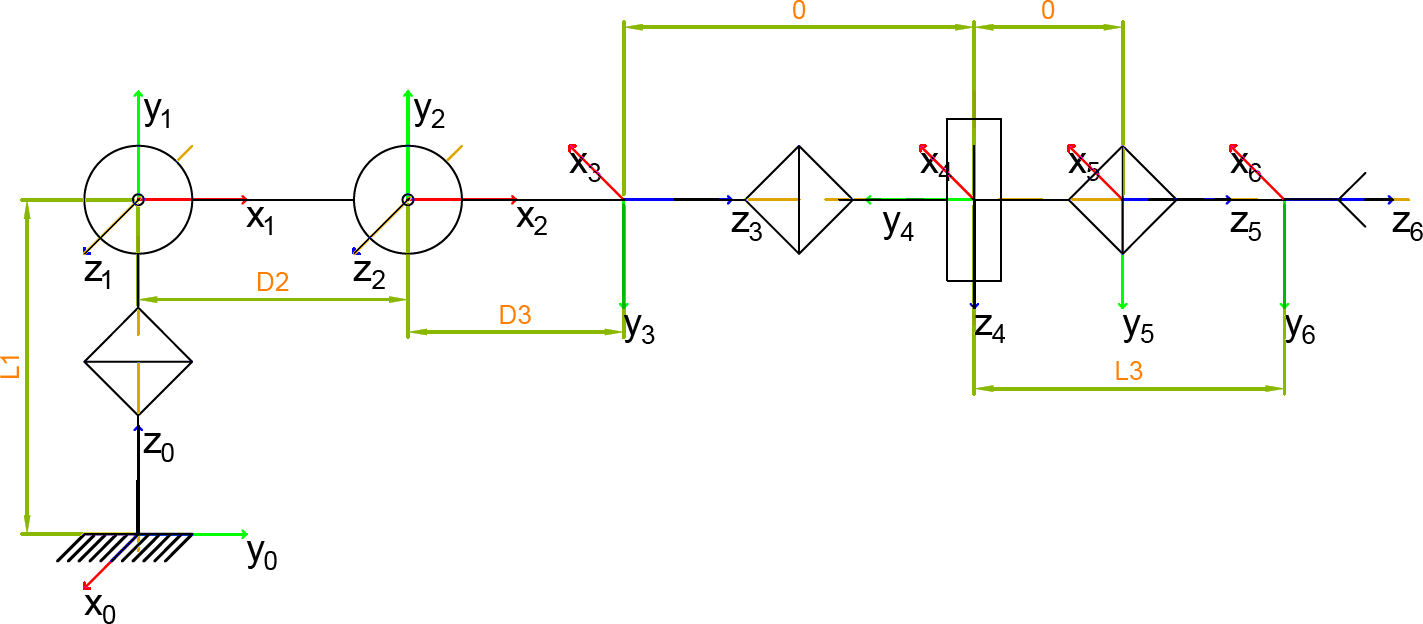
\includegraphics{Sorgenti/Strutture+Polso/Antropomorfo+p.png}
\begin{tabular}{c|c|c|c|c|}
            \cline{2-5} &
            \multicolumn{2}{|c|}{$A_z(\theta,d)$} &
            \multicolumn{2}{|c|}{$A_x(\alpha,a)$} \\
            \hline
        \multicolumn{1}{|c|}{$R_1$} & $q_{1}$ & $0$ & $0$ & $D_{1}$ \\
            \hline
        \multicolumn{1}{|c|}{$R_2$} & $q_{2}$ & $0$ & $0$ & $D_{2}$ \\
            \hline
        \multicolumn{1}{|c|}{$R_3$} & $q_{3}$ & $0$ & $0$ & $D_{3}$ \\
            \hline
\end{tabular}



\end{document}